\documentclass[11pt,a4paper]{article}
\usepackage{od,wrapfig,array}
\usepackage[utf8]{inputenc}
\usepackage[russian]{babel}

\pagestyle{headings}
\title{Кубок ТРИЗ-Саммита – 2020/2021}
\setcounter{tocdepth}{2} 
\author{Трансформация текста в \LaTeX: Hans-Gert Gr\"abe, Leipzig}
\date{November 17, 2020}

\begin{document}
\maketitle
\tableofcontents
\enlargethispage{12em}
\clearpage
\section{Категория 8-10 лет}

\subsection{Номинация «Изобретательство»}

\subsubsection*{Задача 1. Вездеход на Марсе.}
В одном фантастическом рассказе описана экспедиция на Марс. Космический
корабль опустился в долину с очень неровной поверхностью: всюду холмы, ямы,
камни. Космонавты быстро снарядили вездеход – колесный с большими надувными
шинами. Но на первом же крутом склоне вездеход опрокинулся набок. И тут… Нет,
к сожалению, в рассказе изобретатель не появился. А как вы думаете: что бы он
предложил? Учтите, у космонавтов не было возможности переделывать вездеход
(задача из книги Г.С. Альтшуллера «И тут появился изобретатель»).

Проанализируйте контрольное решение (данное в книге): найдите конфликтную
пару, сформулируйте противоречие, ИКР, опишите каким приемом разрешается
противоречие. Предложите другие варианты решения.

\subsubsection*{Задача 2. Водитель для Лунохода.}
Вам нравится управлять моделью гоночного автомобиля с помощью дистанционного
пульта или мчаться на автомобиле-тренажере по сложной трассе? А теперь
представьте, что вы водитель лунохода – настоящего транспортного средства,
способного передвигаться на Луне. В ноябре 1970 г. автоматический корабль
«Луна-17» доставил на спутник Земли первый аппарат, совершивший
непосредственное изучение поверхности Луны. Управление луноходом
осуществлялось группой из 11 человек, составлявших сменные экипажи: командир,
водитель, оператор антенны, штурман, бортинженер. Во время тренировки
водителей на Лунодроме возникла проблема – управление луноходом осуществлялось
по телетрансляции, т.е. водитель видит луноход на телеэкране, а команда,
которую он отправляет выполняется только через 3-5 секунд (время прохождения
сигнала до Луны, обратно и обработка сигнала) – это очень непривычно для
водителя и требует долгой тренировки. Вот один эпизод тренировки: «Включены
двигатели. Луноход рванулся вперед и сразу же замер – водитель приказал ему
остановиться, и машина выполнила приказ. А человек никак не мог объяснить,
почему он прекратил эксперимент, – ему почудилось, что луноход идет в сторону.
Управление по телевидению оказалось не таким простым. Не хватало пространства,
к которому так привыкли глаза. Через 15 минут водитель встал с кресла. И хотя
в комнате было довольно прохладно, его рубашку можно было выжимать – работа у
экрана потребовала огромного напряжения. Проведя несколько часов у экрана,
водитель «вживался» в обстановку, и луноход становился послушным, но на
следующий день все начиналось сначала – появившиеся навыки растворялись».
Ситуация понятна: навыки вождения лунохода по телевизору должны сохраняться
как можно дольше, но проводить все время на тренировке невозможно. Что вы
могли бы предложить водителю лунохода, чтобы в обычной жизни он продолжал
совершенствовать свои навыки дистанционного вождения?  Сформулируйте
противоречия, ИКР, рассмотрите имеющиеся ресурсы.

\subsection{Номинация «Фантазирование»}

\subsubsection*{Задание 1.}
В романе Артура Кларка «Свидание с “Рамой”» описан звездолет инопланетян,
размеры которого достигают 50 километров. Используйте прием «увеличение» и
опишите самый большой звездолет, который сумеете придумать.

\subsubsection*{Задание 2.}
В научно-фантастической повести Генриха Альтова «Третье тысячелетие» описано,
как люди раздробили планету Юпитер в газ и пыль (прием «дробление»). Возникло
огромное облако газа вокруг Солнца. Облако такое же плотное, как атмосфера
Земли. В нем можно летать от планеты к планете на реактивных самолетах и даже
на воздушных шарах. В межпланетном облаке собираются облака и тучи, вспыхивают
молнии. Придумайте рассказ о приключениях детей, отправившихся на воздушном
шаре на Марс.

\subsection{Номинация «Инструменты ТРИЗ»}

\subsubsection*{Задание 1.}
Исследования космоса таят в себе увлекательные приключения, необыкновенные открытия, радость познания неведомого. Есть у этих исследований и чисто практическое применение. Вы, конечно, знаете, что тефлоновое покрытие, беспроводные электроинструменты, геолокационные сервисы и многие другие изобретения, делающие нашу жизнь удобнее и безопаснее, были сделаны в космической промышленности. Задания в номинации «Инструменты ТРИЗ» будут связана именно с таким изобретениями.
\begin{itemize}[noitemsep]
\item[1)] Соберите картотеку «космических изобретений», получивших
  распространение в обычной жизни.
\item[2)] Сформулируйте противоречия, которые решены в данных изобретениях.
\item[3)] Предложите необычное использование этих изобретений для решения еще
  не поставленных задач.
\end{itemize}

\subsubsection*{Задание 2.}

Сказки, мифы, легенды – часто это единственная возможность узнать, как жили
наши далекие-далекие предки. А ведь так интересно, что происходило на нашей
Земле много веков назад, какие рассказывали истории, какие были дома, о чем
думали, о чем мечтали наши прародители. А вы хотели бы, чтобы о вашей семье, о
ваших друзьях, о вашем городе узнали люди через много тысячелетий?  Придумайте
сказку, миф, легенду, фантастический рассказ такой интересный, чтобы его
рассказывали и сотни лет спустя.

\subsection{Номинация «Исследования»}

\subsubsection*{Задание 1.}

\newcommand{\AnimalsInCosmos}{С самого начала освоения космоса человека
  сопровождали (а иногда заменяли) животные. За более чем 60 лет космических
  исследований в космосе побывали самые разные животные. Интереснейшие
  эксперименты, организованные на орбите, связаны с выращиванием
  растений. Далеко не сразу удалось создать условия, в которых растения не
  только наращивали зеленую массу, но и цвели и плодоносили. Итак,
  исследовательская тема: «Животные и растения в космосе». Вы можете выбрать
  для своего исследования более конкретную тему.
\begin{itemize}[noitemsep]
\item Картотека «Животные в космосе». Вид животных, дата полета в космос,
  продолжительность пребывания в космосе, цели эксперимента, результаты
  эксперимента.
\item Картотека «Растения в космосе». Вид растения, дата полета в космос,
  продолжительность пребывания в космосе, цели эксперимента, результаты
  эксперимента.
\item Картотека «Устройства для поддержания жизнедеятельности животных в
  космосе». Какие задачи и как решались в каждом из этих устройств.
\item Картотека «Устройства для поддержания жизнедеятельности растений в
  космосе». Какие задачи и как решались в каждом из этих устройств.
\item Какие задачи по адаптации животных и растений для пребывания в космосе
  все еще не решены? Предложите их возможные решения.
\end{itemize}}

\AnimalsInCosmos

\subsection{Номинация «Видеоролики по ТРИЗ»}

\newcommand{\VideoOne}{Есть ли в вашем городе места, связанные с исследованием
  космоса? Сделайте репортаж о посещении музея, выставки, научного
  центра. Попробуйте взять интервью у специалистов, связанных с космическими
  исследованиями. }

\newcommand{\VideoTwo}{Проиллюстрируйте с помощью средств
  кино или анимации решение изобретательских задач. Придумайте истории, в
  которых возникает проблема, постарайтесь подробно прокомментировать в чем
  состоит противоречие, какое идеальное решение необходимо достичь, какие
  приемы использованы для решения.}

\newcommand{\GeneralText}{Ролики должны быть короткие (от 2-х до 10 минут).
  Должны быть указаны все авторы этого сюжета: автор сценария, оператор,
  монтажер, актеры и т.д.  Данная работа направлена на формирование
  методического материала для обучения ТРИЗ. На сайте ТРИЗ Саммита
  опубликованы видеоролики, представленные на прошлый Кубок ТРИЗ Саммита:\\
  \url{http://triz-summit.ru/ru/contest/competition/video/}\\
  \url{https://www.youtube.com/channel/UCjMNOjboWRBQA72DJvaC7ew/featured}

  В подготовке заданий Кубка ТРИЗ Саммита-2020/2021 принимали участие Рубин
  М.С., Рубина Н.В., номинация «фантазирование» подготовлена П.Р. Амнуэлем.
}

\subsubsection*{Задание 1.}\VideoOne
\subsubsection*{Задание 2.}\VideoTwo

\GeneralText
\clearpage

\section{Категория 11-14 лет}

\subsection{Номинация «Изобретательство»}

\subsubsection*{Задача. Мягкая посадка на Марс.}

\begin{wrapfigure}{r}{.3\textwidth}\vspace*{-1em}\centering
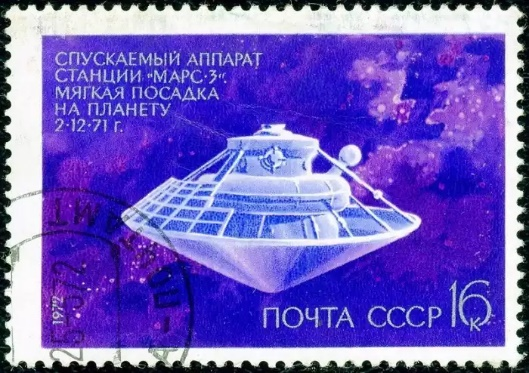
\includegraphics[width=.25\textwidth]{jEMlaM.jpg}
\end{wrapfigure}
Мечтой многих исследователей космоса остаётся полет на Марс. Первым
искусственным объектом, коснувшимся поверхности Красной планеты, стал марсоход
ПрОП-М (Прибор оценки проходимости - Марс). Мягкая посадка произошла 2 декабря
1971 года. Попробуем пройти часть пути до Марса вместе со спускаемым
аппаратом, марсоходом и его конструкторами. Итак, спускаемый аппарат достиг
границы атмосферы Марса, начинается аэродинамическое (воздушное)
торможение. Для осуществления мягкой посадки задействуется система парашютов.

\subsubsection*{Задача 1.}
Для начала работы парашютной системы нужно задействовать вытяжной парашют – он
имеет небольшой размер, но создает необходимую тягу для полного раскрытия
основного парашюта. Вытяжной парашют должен раскрыться не раньше и не позже
момента вхождения спускаемого аппарата в атмосферу Марса. Что может быть
сигналом для срабатывания порохового двигателя на крышке вытяжного парашюта?
(сформулируйте ИКР и рассмотрите ресурсы)
\begin{center}
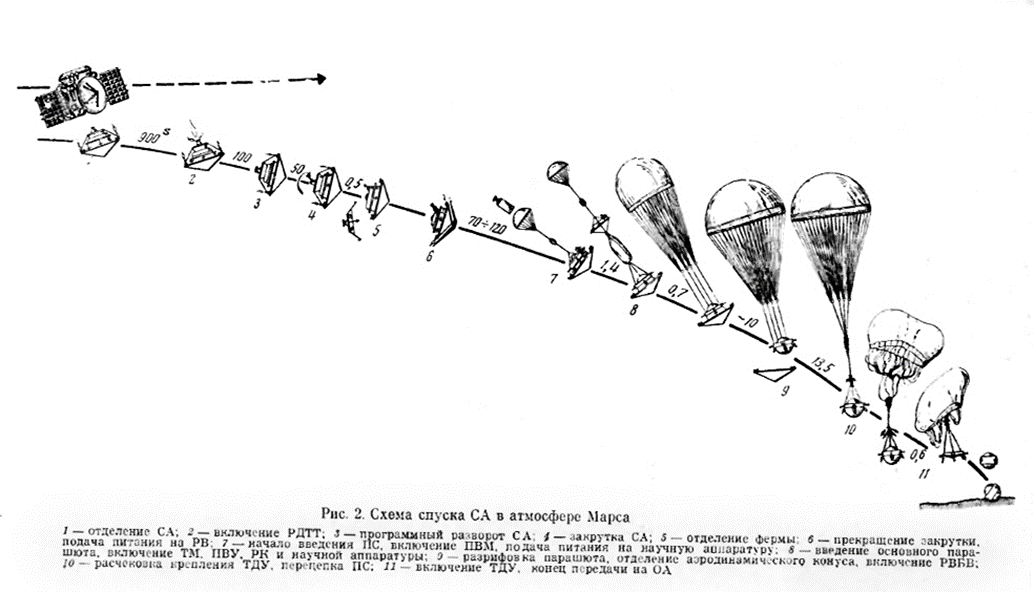
\includegraphics[width=.95\textwidth]{12uaYg.png}
\end{center}

\subsubsection*{Задача 2.}
Следующий этап — ввод и раскрытие основного парашюта. Необходимо реализовать
несколько операций: вскрыть парашютный отсек, удалить верхнюю крышку, провести
полное раскрытие основного парашюта и, наконец, не допустить, чтобы основной
парашют накрыл собой станцию. Проанализируйте тормозную систему спускаемого
аппарата, выделите нежелательные эффекты, возникающие при торможении,
сформулируйте противоречия. Какие устройства задействованы в устранении
нежелательных эффектов?
\begin{center}
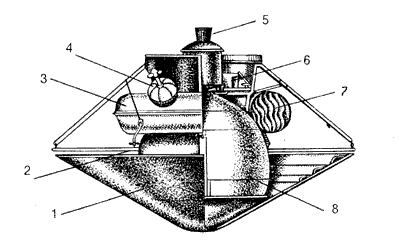
\includegraphics[width=.4\textwidth]{GIj0Ml.png}\hfill
  \begin{minipage}[b]{.55\textwidth}\small
    Спускаемый аппарат станции "Марс-2":
    \begin{itemize}[noitemsep]
    \item[1] — аэродинамический конус;
    \item[2] — антенна радиовысотомера;
    \item[3] — парашютный контейнер;
    \item[4] — двигатель ввода вытяжного парашюта;
    \item[5] — двигатель увода спускаемого аппарата;
    \item[6] — приборы и аппаратура системы управления;
    \item[7] — основной парашют;
    \item[8] — автоматическая марсианская станция
    \end{itemize}
  \end{minipage}
\end{center}
Эта история имеет неожиданное и интересное продолжение.

\subsubsection*{Задача 3.}
Вы никогда не задавались вопросом, что известно об отработавших аппаратах,
оставшихся на Луне, Марсе, Венере? Исследования результатов разумной
деятельности на планетах и их спутниках пока не оформилось в самостоятельную
область, но публикаций по направлению «космическая археология» уже достаточно
много. Казалось бы, места посадок всех аппаратов, исследовавших планеты и
спутники точно известны, но… вот как описывает эту задачу Виталий Егоров:
«Обратившись к сайту HiRise, я обнаружил только снимок 2007 под названием
Center of Soviet Mars 3 Landing Ellipse. Это было для меня открытием,
поскольку я так был уверен во всемогуществе NASA и HIRise, что ожидал увидеть
точное указание, где стоит наша станция. Беглый поиск в сети тоже не дал
результата. Т.е. было очевидно, что Марс-3 так и не найден. Я скачал
полноформатный снимок (1,3 гб), открыл его и понял, почему за 5 лет так никто
и не отыскал станцию. (Снимок имеет разрешение 30 см на пиксель, т.е. объект
размером 30 см представляет собой 1 точку. «Марс-3» - объект размером 1,5 м –
на снимке это объект 6Х6 точек). Представьте себе поиск на прямоугольнике 6 на
20 километров округлого объекта шириной 1,5 метра. Знаю, многие сейчас
подумали, что надо было написать программу, которая сама бы искала станцию. Но
думаю, такой поиск невозможен, пока не создан искусственный интеллект. Да,
программа могла бы выделить интересные валуны соответствующего размера. Но там
таких объектов — тысячи, поскольку рядом кратер, из которого веером
разлеталась порода».

Что бы вы предложили в этой ситуации? Как найти «Марс-3»? И главное, зачем
исследовать результаты разумной деятельности (деятельности людей) на планетах
и спутниках, какую информацию можно получить?

\subsubsection*{Задача. Опасная планета.}
В одном фантастическом рассказе описана удивительная планета. Все на ней, как
на Земле: такая же атмосфера, такие же растения и животные. Но насекомые и
птицы летают со сверхзвуковой скоростью. Не будем уточнять, как им это
удается. Суть дела в другом. Вы, наверное, знаете, что столкновение самолетов
с птицами приводит к авариям. А тут воздух наполнен живыми «пулями» и
«снарядами»… Высадили двух космонавтов – и едва удалось их спасти. Даже
бронированный вездеход был быстро разрушен сверхзвуковыми «мухами»…
Представьте себя участником экспедиции к такой планете. Предложите, как
обезопасить себя и экипаж.

Представим обратную ситуацию. На изучаемой нами планете обнаружена разумная
жизнь. Однако скорость изменений, скорость реакций разумных существ замедлена
по сравнению с людьми во много раз. То, что для человека мгновение – для
инопланетянина годы. Как наладить контакт, как провести переговоры?

\subsection{Номинация «Фантазирование»}

\subsubsection*{Задание 1.}
В наши дни космонавты выходят в космическое пространство в скафандрах, которые
дают возможность дышать и защищают от радиации. Может ли человек жить в
космосе без скафандра? В реальности – пока нет, но фантасты писали о том, как
это может получиться. Придумайте и вы. Воспользуйтесь одним из приемов
фантазирования.

\subsubsection*{Задание 2.}
В романе Хола Клемента «Экспедиция “Тяготение”» действие происходит на
планете, где сила тяжести в 800 раз больше земной. Придумайте фантастическую
планету, отличающуюся от Земли каким-нибудь другим параметром. Опишите
приключения экипажа звездолета на такой планете.

\subsection{Номинация «Инструменты ТРИЗ»}

\subsubsection*{Задание 1.}

\newcommand{\CosmicInventions}{Космические путешествия и исследования – мечта
  многих поколений смелых людей. Есть у этих исследований и чисто практическое
  применение. Вы, конечно, знаете, что тефлоновое покрытие, беспроводные
  электроинструменты, геолокационные сервисы и многие другие изобретения,
  делающие нашу жизнь удобнее и безопаснее, были сделаны в космической
  промышленности. Задания в номинации «Инструменты ТРИЗ» будут связана именно
  с таким изобретениями.
\begin{itemize}[noitemsep]
\item[1)] Соберите картотеку «космических изобретений», получивших
  распространение в обычной жизни.
\item[2)] Сформулируйте противоречия, которые решены в данных изобретениях.
\item[3)] Предложите необычное использование этих изобретений для решения еще
  не поставленных задач.
\end{itemize}}

\CosmicInventions

\subsection{Номинация «Исследования»}

\subsubsection*{Задание 1.}

\AnimalsInCosmos

Возможно ли создание на орбите условий, похожих на сложные природные системы,
такие как лес, луг и т.д., где животные и растения взаимодействуют друг с
другом? Существуют ли подобные проекты, какие проблемы возникают при их
реализации?

\subsubsection*{Задание 2.}
В каждой семье есть истории, передающиеся из поколения в поколение: от деда,
который приехал из Чикаго в Россию, от бабушки, которая спасала жизни на
фронте и т.д. Бывают случаи трагичные, бывают смешные, но все они запоминаются
своей яркостью, их с удовольствием пересказывают по много раз, передают от
отца к сыну. Реальные истории обрастают легендарными подробностями. Опишите
историю своей семьи: с каких времен, и из каких мест берет начало ваша семья,
какие особые поступки совершили ваши предки, какие особые истории сопровождали
вашу семью. Напишите то, чем вам хотелось бы поделиться о вашей семье.
Закончив рассказ о вашей семье, сделайте комментарий к этой истории,
представьте себе, что ваш рассказ прочитали в XXV веке, и ничего другого о
нашей эпохе им неизвестно. Как будет выглядеть наша цивилизация, если ее будут
изучать только на основе истории вашей семьи? Что бы вы изменили в своем
рассказе, чтобы его поняли люди через многие века?
\clearpage

\subsection{Номинация «Видеоролики по ТРИЗ»}
\subsubsection*{Задание 1.}\VideoOne
\subsubsection*{Задание 2.}\VideoTwo

\GeneralText
\clearpage

\section{Категория 15-17 лет}

\subsection{Номинация «Изобретательство»}

\newcommand{\Aberration}{Известно, что при преломлении солнечный свет
  разлагается на спектр. От этого очень страдали астрономы. В линзах телескопа
  свет от Солнца, планет и звезд тоже преломляется. И космические объекты
  оказываются окруженными разноцветными ореолами, что мешает их как следует
  рассмотреть. Это явление называется «хроматической аберрацией». Великий
  английский физик И. Ньютон считал, что от нее избавиться невозможно.
  Предложите способ изготовления линз, не дающий хроматическую аберрацию.}

\newcommand{\CosmicOperation}{Хотя в космонавты принимают исключительно
  крепких и здоровых людей, на космических станциях ближайшего будущего с ними
  всякое может случиться. Не исключено, что придется делать сложную
  операцию. На Земле больного кладут на операционный стол, где и больной, и
  стол, и инструменты и врачи удерживаются в одном положении силой тяжести. Но
  в невесомости это будет не так просто. На первый взгляд, стол можно
  привинтить к полу. Но врачей не привинтишь. Они должны передвигаться. Не
  привинтишь и инструменты, и посуду с препаратами. Больного тоже не всегда
  можно привязывать – мало ли какие травмы он получил. А если операция
  серьезная, требует широкого вскрытия, то удерживать от «полетов» придется и
  внутренние органы оперируемого. Предложите конструкцию операционной комнаты,
  операционного стола, инструментов и приспособлений для самых разнообразных
  операций в условиях невесомости.}

\subsubsection*{Задача 1.}\Aberration
\subsubsection*{Задача 2.}\CosmicOperation

\subsection{Номинация «Фантазирование»}

\subsubsection*{Задание 1.}
В «этажной схеме» Г. Альтшуллера существует четыре способа («этажа»), с
помощью которого можно придумать новую фантастическую идею. Изучите эту схему.
Придумайте и опишите идеи третьего и четвертого этажей для объекта «скафандр».

\subsubsection*{Задание 2.}
В фантастическом романе Ларри Нивена «Интегральные деревья» люди живут на
планете, которая представляет собой огромное дерево, летающее в космосе по
орбите вокруг звезды, похожей на Солнце. В романе Пола Шеффилда «Мир – кольцо»
люди живут на поверхности огромного кольца, вращающегося вокруг звезды.
Придумайте и опишите фантастическую планету, используйте для этого
какой-нибудь прием фантазирования. Напишите небольшой рассказ о приключениях
на придуманной вами планете.

\subsection{Номинация «Инструменты ТРИЗ»}

\newcommand{\BlackBox}{С помощью морфологической таблицы (см. «краткий анализ
  задачи «О черном ящике цивилизации») сформулируйте исследовательскую тему,
  подзадачу для задачи о “черном ящике” цивилизации. Соберите примеры, задачи
  по выбранной вами теме. Проанализируйте собранную информацию. Какие способы
  передачи информации о современной цивилизации вы можете предложить? Что,
  по-вашему мнению, можно сделать сегодня для сохранения информации о нашей
  цивилизации?}

\subsubsection*{Задание 1.}\BlackBox
\subsubsection*{Задание 2.}\CosmicInventions

\subsection{Номинация «Исследования»}

\newcommand{\BlackBoxOfCivilization}{
\subsubsection*{Задача о “черном ящике” цивилизации.}
(цитируется по: Г.С. Альтшуллер, И.М. Верткин, “Как стать еретиком. Жизненная
стратегия творческой личности”, задачник; сборник “Как стать еретиком”,
Петрозаводск, “Карелия”, 1991 г., стр. 166-168).

“В крупных современных самолетах встроен так называемый “черный ящик”. Он
предназначен для записи режимов полета. В случае аварии легко выяснить ее
причины, установить виновных. Если авария произошла по вине летчиков или из-за
недостатков конструкции самолета, анализ записи позволяет будущие полеты
сделать безопаснее. Предотвратить происходящую аварию, помочь терпящим
бедствие “черный ящик” не способен, да это и не входит в его функции. Главная
его цель – работа на “завтра”; “черный ящик” позволяет учиться на чужих
ошибках.

В последнее время этими устройствами стали снабжать и океанские
лайнеры. Очевидно, в недалеком будущем “черные ящике” станут обязательными
атрибутами всех видов общественного транспорта, а, возможно, и личных
мото-транспортных средств.

Во все времена люди, отправлявшиеся в отчаянные путешествия, готовящиеся к
трагическим событиям, старались передать потомкам свой опыт, свое описание
происходящего. Обычно такие записи велись в трагических периоды людей: в
осажденных городах, в тюремных застенках, в ожидании близкой смерти. Вспомните
кумранские рукописи, дневник полярной экспедиции Скотта, записи самонаблюдений
Алена Бомбара.

Как правило, подобные “завещания” начинают составлять в последний момент,
когда остро ощущается нехватка времени и подходящих условий. Поэтому мы
знакомы лишь с единичными записями, чудом дошедшими до нас. Ко всему, - в том
числе (а может быть, в первую очередь) и к катастрофам, - надо готовиться
заранее.

Наша Земля не менее уязвима, чем любой другой “общественный вид транспорта”. В
прежние времена причиной будущего “конца света” считались некие мистические
силы “свыше”. В недалеком прошлом эту роль передали таинственным космическим
пришельцам, враждебно настроенным к землянам. Сейчас говорят, что главный наш
враг – мы сами, и предрекают генетический, социальный, демографический,
ядерный, экологический и прочие подобного рода кризисы. В общем-то, неважно, в
результате чего может произойти катастрофа, по этим или по еще неведомым
причинам; главное, что это в принципе возможно. Значит, Земле необходим свой
“черный ящик”. Он должен зафиксировать истинные причины возможной трагедии,
сохранить запись в целости нужное время и передать ее будущим поколениям:
опыт, особенно столь отрицательный и глобальный, бесценен.

Только будущее может однозначно ответить на вопрос о сегодняшней актуальности
“черного ящика” для планеты. Одно можно сказать уверенно уже сейчас: эта
проблема не надумана. Если она не “горящая”, - прекрасно, значит, у нас есть
время спокойно, тщательно подготовиться к ее решению. Если времени в обрез, -
что ж, надо успеть сделать то, что еще можно успеть. Словом, чем раньше
начнется разработка этой проблемы, тем лучше.

Решение проблемы во многом зависит от масштабов вероятной катастрофы. Возможно
несколько вариантов:
\begin{itemize}[noitemsep]
\item[а)] В результате катастрофы исчезнет половина населения Земли. Связь
  между городами сохранится. В какой-то степени сохранится прежняя
  инфраструктура.
\item[б)] На Земле останется несколько десятков тысяч человек. Связи
  практически не будет никакой. Остатки населения довольно быстро деградирует,
  к примитивным ремеслам, к примитивной технике. Пройдет много времени, прежде
  чем вновь возникнут условия для ощутимого рывка вперед.
\item[в)] Разумная жизнь вовсе исчезнет с лица Земли. Лет через 100-150
  возникнут условия, приемлемые для жизни человека, но, когда произойдет
  возрождение Разума – “одному аллаху ведомо”.
\item[г)] С Земли исчезнет всякая жизнь. Время восстановления условий –
  миллиард лет.
\end{itemize}
Давайте остановимся на самом трудном – последнем варианте. Если удастся
придумать что-то для преодоления обостренного конфликта, в более мягких
условиях задача тем более будет решена.

Итак, условия проблемы. Через 100-150 лет произойдет исчезновение всякой жизни
с Земли. Возможное время восстановления - миллиард лет. Как передать “черный
ящик” на такую временную дистанцию? Что в него записать?

Это очень сложные вопросы. Например, вопрос о технике передачи
информации. Ведь сегодня неизвестно – кому придется передать информацию: кто
знает, какой вид примет разумная жизнь через миллиард лет после нашей эры… Да
и возникнет ли она самостоятельно на Земле? Как помочь в восстановлении
разумной жизни? Как сохранить генофонд нашей флоры и фауны? Как сделать так,
чтобы информация попала вовремя: когда уже были бы способны понять, о чем идет
речь, и еще было бы не поздно? Как сделать так, чтобы информацию смогли без
труда расшифровать? Как сохранить запись на такой временной дистанции? Как
сделать так, чтобы информации поверили, чтобы не восприняли ее как глупую
шутку соотечественников?

Не менее не ясен пока и вопрос о содержании “черного ящика”. Скорее всего,
“ящик” должен состоять из двух частей: “оперативной” (о причинах аварии) и
“стационарной” (о накопленной культуре, знаниях на Земле). Как постоянно
пополнять “оперативную” часть, включая непосредственно момент и последующее
время? Что записать в “стационарную” часть? “Все знания мира”? Что конкретно?
Каковы критерии отбора? Какие рекомендации мы можем передать будущей разумной
жизни для предотвращения аналогичных трагедий?

Вопросов много…

Чем хороша проблема? “Передача информации” на сегодня – тема для
первооткрывателя, абсолютно свободная от конкуренции, по крайней мере, на
ближайшие 30-50 лет (надеемся, что разум все-таки возобладает и человечество
осознает проблему раньше случившейся катастрофы). Это одна из немногочисленных
тем, полностью лишенных отрицательной стороны. Тема максимально
благородная. Предельно общественно-полезная. Супермасштабная – совершенно
очевидно уже сейчас, что эта тема на всю жизнь, причем не на одну. Тема имеет
социальный и технический аспекты, т.е. подходит для человека с любой
специализацией.

(Заранее можно предсказать типовое ханжеское возражение против этой проблемы:
когда горит дом, надо не записывать, отчего произошел пожар, а таскать ведра с
водой. Возможная катастрофа цивилизации ставит много проблем, большинство из
которых воспринимается пока весьма абстрактно. Основная часть населения
планеты продолжает работать на предприятиях своих государств, т.е. продолжает
участвовать в уничтожении природы. Немногие бьют в колокола и пытаются тушить
разгорающееся пламя. Но никто, ни один человек на всей Земле даже близко не
подошел к проблеме “черного ящика”! Как знать, возможно, письмо, отправленное
на миллиард лет вперед, важнее двух сегодняшних ведер воды…)”.}

\BlackBoxOfCivilization

\subsection{Номинация «Видеоролики по ТРИЗ»}

\newcommand{\VideoThree}{Проиллюстрируйте с помощью средств кино или анимации
  решение изобретательских задач. Это могут быть как технические решения, так
  и изобретения в нетехнических областях. }

\subsubsection*{Задание 1.}\VideoOne
\subsubsection*{Задание 2.}\VideoThree

\GeneralText
\clearpage

\section{Категория студенты}

\subsection{Номинация «Изобретательство»}

\subsubsection*{Задача 1.}\Aberration
\subsubsection*{Задача 2.}\CosmicOperation

\subsection{Номинация «Фантазирование»}

\subsubsection*{Задание 1.}
В цикле романов Грега Игана «Ортогональная вселенная» действие происходит во
вселенной, где скорость света зависит от длины волны. Придумайте и опишите
вселенную, в которой изменен какой-нибудь другой физический закон или мировая
постоянная.

\subsubsection*{Задание 2.} 
В цикле романов Стивена Бакстера и Терри Пратчетта «Бесконечная Земля» описаны
миры, в каждом из которых существует Земля, отличающаяся от нашей планеты тем,
что на каком-то этапе эволюция пошла иначе, чем в нашей реальности. В одном
случае динозавры не погибли, в другом вся планета оказалась покрытой лесами, в
третьей нет людей, но есть разумные собаки…  Придумайте космический фактор,
который когда-то изменил ход эволюции на Земле, и опишите, какой в результате
действия этого фактора стала планета в наши дни.

\subsection{Номинация «Инструменты ТРИЗ»}

\subsubsection*{Задание 1.}\BlackBox
\subsubsection*{Задание 2.}\CosmicInventions

\subsection{Номинация «Исследования»}

\BlackBoxOfCivilization

\subsection{Номинация «Видеоролики по ТРИЗ»}

\subsubsection*{Задание 1.}\VideoOne
\subsubsection*{Задание 2.}\VideoThree

\GeneralText
\clearpage

\section{Краткий анализ задачи о “черном ящике” цивилизации. }
\begin{center}
  © Рубин М.С.
\end{center}
Задача о “черном ящике” цивилизации была предложена как генератор новых
исследовательских тем, источник Достойной Цели для исследователей.  

“Г.С. Альтшуллер и И.М. Верткин выделяют три яруса тем:
\begin{itemize}[noitemsep]
\item темы узкотехнические, узко-научные, узко-художественные, например,
  изобретение ракет;
\item темы общетехнические, общенаучные, общехудожественные, например,
  развитие космонавтики;
\item темы, затрагивающие цивилизацию в целом (социально-технические,
  социально-научные, социально-художественные и пр.), например, проектирование
  космической цивилизации или цивилизации с телевидением.
\end{itemize}
С исследовательской точки зрения эффективнее всего работать с темами третьего
яруса - на уровне общечеловеческих проблем. Здесь самый большой простор для
развития тем, наименьшая вероятность "застрять" на мелкотемье или оказаться в
ситуации острой конкуренции с другими исследованиями. В качестве примера мне
хотелось представить хотя бы одну проблему общечеловеческого уровня. Речь
пойдет о проблеме создания "черного ящика" на случай всемирной катастрофы.
("Как стать еретиком", Карелия, 1991, стр. 166-168).

Очень не многие из специалистов по ТРИЗ работали над предложенной задачей, еще
меньше публикаций на эту тему. Задача сложная и мы решили предложить некоторые
подходы к ней. Это лишь наш взгляд, и мы не претендуем на то, что это
единственный подход к задаче о “черном ящике” цивилизации.

Нам сразу хотелось бы отсечь очевидно слабые решения. Например: создание
глобальных систем сбора информации от каждого жителя Земли и размещение ее на
каком-нибудь спутнике Земли или Венеры. Не смотря, на очевидность
невыполнимости, не идеальности, подобные идеи все равно
высказываются. Исследовательская тема будет тогда интересной и сильной, когда
она будет направлена на разрешение противоречий, заложенных в задаче о “черном
ящике” цивилизации (например, информации должно быть очень много, чтобы
отразить все стороны цивилизации, и должно быть мало, чтобы ее легче было
сохранить и донести до потомков; или место хранения информации должно быть
близко, чтобы легче было размещать информацию, и должно быть далеко, чтобы
информация надежнее сохранялась при катастрофе), и максимально приближаться к
идеальному конечному результату (например, катастрофическая сила, разрушающая
цивилизацию САМА сохраняет ее для потомков).

Во время конференции школьников и студентов по ТРИЗ “ИКАРиада-2001” была
предложена морфологическая таблица для анализа задачи:

\begin{center}\small
  \begin{tabular}{|*{6}{>{\raggedright}p{1.9cm}|}c|}\hline
1. Какой объект & 1.1 Семья & 1.2. Дом & 1.3. Город & 1.4 Страна & 1.5. Весь
мир & \ldots \\\hline
2. Кому, куда & 2.1. Другим людям & 2.2. Другому государству & 2.3. Потомкам
через 50 (100, 1000) лет & 2.4. Иноземным цивилизациям & 2.5. Необитаемой
планете & \ldots \\\hline
3. Цель & 3.1. Сохранить информацию & 3.2. Избежать ошибок & 3.3. Сохранить
цивилизацию & 3.4. Возродить цивилизацию & 3.5. Расширить границы цивилизации
& \ldots \\\hline
4. Ресурсы & 4.1. Ресурсы сохраняемой системы & 4.2. Ресурсы уничтожающей силы
& 4.3. Ресурсы современной внешней среды & 4.4. Ресурсы среды, в которую
попадает “Черный ящик” & \ldots & \\\hline 
5. Причина катастрофы & 5.1 Естественные & 5.2. Социальные конфликты &
5.3. Природные катаклизмы & 5.4 Межличностные конфликты & 5.5. Террор и
преступления & \ldots \\\hline
  \end{tabular}
\end{center}
Эта таблица может быть использована для формулировки множества подзадач,
например, вариант (1.3-2.3-3.2-4.1-5.1) может быть сформулирован следующим
образом: как сохранить информацию о современном Петрозаводске для поколения
людей 22-го века в целях избегания повторения допущенных ошибок силами самого
города, если он будет изменяться в результате естественной эволюции. Уровень
формулированных задач и их остроту можно изменять по собственному вкусу.

Имеется очень широкий выбор направлений ведения дальнейших исследовательских
работ по теме “черного ящика цивилизации”. Можно, например, уточнить оси
морфологического ящика: их количество и содержание. Можно сделать подборку
конкретных задач, собранных в рамках общей темы “черного ящика
цивилизации”. Можно провести анализ каждой из подзадач: сформулировать
противоречия, ИКР, проанализировать ресурсы. Можно выстроить иерархию задач
темы “черного ящика цивилизации”. Можно собрать информацию о наиболее частых
причинах гибели цивилизаций. Очень плодотворным может стать анализ методов
восстановления информации, которые имеются в археологии и у
историков. Возможностей для ведения исследовательской работы, действительно
очень много.

Очень эффективным можно считать сбор различных картотек (см. статью М. Рубина
“Личные картотеки – фундамент творчества”, статья опубликована на сайте
ОТСМ-ТРИЗ-технологий  \url{http://www.triz.minsk.by/e/221001.htm} ) по теме
“черного ящика цивилизации”.

Можно, например, начать с картотеки "черных ящиков" - с самолетов разного
типа, океанских лайнеров или других систем. Любопытно выяснить характер
фиксируемой информации, основные проблемы и противоречия "черных ящиков",
сделать прогноз их развития. Может оказаться, например, что "Черный ящик
цивилизации" - логическое продолжение развития обычных "черных
ящиков". Попутно можно предложить новые идеи и решения в этой области.

Очень важный вопрос: что именно передавать потомкам или пришельцам о погибшей
цивилизации. Для ответа на него может оказаться другая картотека - о КЛЮЧЕВЫХ
НАХОДКАХ (памятников), помощью которых удалось раскрыть тайны погибших
цивилизаций.
\medskip

Приведу только один пример. Для изучения погибшей цивилизации майя очень важно было расшифровать письменность этого народа. Сделать это удалось, главным образом, с помощью двух документов:
\begin{itemize}
\item рукописи "Сообщение о делах в Юкатане" времен завоевания испанцами
  индейцев майя, где, в частности, приводился сокращенный алфавит майя с его
  "ОЗВУЧИВАНИЕМ" ИСПАНСКИМИ буквами;
\item записям древних мифов (книги Чилам Балам), сделанных в XVI веке
  ЛАТИНСКИМИ БУКВАМИ и отражающих язык майя времен начала нашей эры.
\end{itemize}
К этому, безусловно, необходимо добавить дошедшие до нас современные (живые)
языки майя и испанцев, а также сведения об испанском языке ХYI века.

Любопытно отметить, что "черные ящик" цивилизации майя дошел до нас в виде
бисистемы: в первую очередь это сами города древних майя с храмами, надписями
на них, картинками, рисунками, а также ключ к их объяснению - алфавит, о
котором мы только что упоминали.
\medskip

При самом трудном варианте (с Земли исчезает всякая жизнь) живой язык,
естественно, не сохранится. Так, например, произошло с шумерскими текстами: их
удалось полностью расшифровать, но никто не знает, как звучал этот
язык. Необходимо совмещение предмета или действия (показанных в различных
ситуациях) с его письменным и звуковым (речевым) изображением. Что-то вроде
телевизионных комиксов для изучения иностранных языков.

Пример "черного ящика" цивилизации древних майя наводит на интересную
мысль. Дело в том, что рукопись "Сообщение о делах в Юкатане" - основной,
наиболее полный и точный документ о древней цивилизации - была составлена
епископом-испанцем Диего де Ланда. Именно под его руководством тщательнейшим
образом было уничтожено почти все письменно и другое культурное наследие майя
(за эту свою деятельность де Ланда и получил звание епископа). Рукопись де
Ланды - своеобразный отчет перед начальством о проделанной "работе" по
истреблению ереси. Возникает любопытная гипотеза: причина, приводящая к
катастрофе (например, испанцы в лице Диего де Ланды) САМА создает "черный
ящик" (знаменитую рукопись епископа). Второй документ-ключ к разгадке текстов
майя - "Книги Чилам Балам", написанные на латинице - имеют примерно такой же
характер происхождения, как и рукопись де Ланды. Испанцы запрещали майя
пользоваться родной письменностью, и те стали записывать древние тексты на
дозволенной латинице. Все та же ситуация: испанцы, своими запретами, САМИ
вынудили майя создать документ о своей культуре, понятный для потомков. Еще
один пример, о котором мы уже вспоминали: извержение Везувия уничтожило
Помпеи, но оно же и сохранило для нас этот город, засыпав его толстым слоем
пепла.
\medskip

Итак, сила, приводящая к катастрофе, САМА создает "черный ящик" в момент
катастрофы. Что это - гипотеза, идеальный вариант решения проблемы или
закономерность образования "черных ящиков" цивилизаций? Ответить на этот
вопрос поможет картотека КЛЮЧЕВЫХ НАХОДОК к разгадке культуры погибших
цивилизаций: с помощью чего удалось расшифровать информацию о жизни людей. В
связи с этим можно вспомнить и о многочисленных примерах ключевых находок
древних животных: мамонтов, неандертальцев, динозавров.

Общеизвестна, например, находка очень хорошо сохранившегося динозавра из рода
аллозавров. Эта находка стала настолько важной для науки, что останки этого
динозавра назвали по имени – Большой Ал. Хорошо сохранился не только скелет,
но отпечаток сердца. Ученым удалось восстановить с абсолютной точностью
особенности поведения аллозавров, среду их обитания, скорость передвижения,
повадки. Удалось даже сделать жизнеописание Большого Ала: в каком возрасте,
какие травмы он получил, в каких ситуациях эти травмы и болезни могли
возникнуть, от чего умер этот динозавр, живший 45 миллионов лет назад. Уже
старый и больной Большой Ал отправился к реке во время засушливого
лета. Дождей не было, и вода все не приходила. Обессиленный, он ждал воду в
русле высохшей реки. Вскоре вода пришла, но Большой Ал уже умер. Ил обволок
тело и сохранил его для нас на многие миллионы лет. Река, убившая динозавра,
САМА же сохранила информацию о нем.
\medskip

Возможно, что с помощью одной только разрушающей цивилизацию силы не удастся
найти абсолютно надежный механизм создания в нужный момент "черного
ящика". Тогда возникает новая задача: как сделать, чтобы "черный ящик" был
полезен и необходим при нормальном течении жизни без катастроф. Это позволило
бы сделать весь проект создания "черного ящика" цивилизации гораздо дешевле,
повысило бы вероятность его реализации, обеспечило бы надежность его
функционирования в до катастрофический период.

Как и всякая сверхпроблема, проект "Черный ящик" дает целый спектр задач,
проблем и тем для исследования. Представлю еще одну из них, но прежде -
карточка из моей картотеки:

"Кто спасется в катастрофе".

"С момента вступления в ядерную эпоху перед сверхдержавами постоянно стоит
дилемма - чье выживание обеспечить в первую очередь в случае крупномасштабного
конфликта: населения страны или высших эшелонов власти? В самом начале своего
восьмилетнего пребывания у власти президент Рейган, отбросив предрассудки
"холодной войны" с ее ориентацией на гражданскую оборону, заявил, что в
ядерной войне можно победить, но лишь в том случае, если будет обеспечено
выживание высших гражданских и  военных руководителей. Процедура эвакуации
предусмотрена для представителей высших эшелонов власти, выживание которых
считается необходимым для "обеспечения непрерывности государственной власти" -
всего для более 1000 человек".  ("Комсомольская правда", 26.08.1989).

Аналогичные программы имеются не только в США, но и в других странах. В
результате реализации подобных проектов вполне возможна ситуация, при которой
после катастрофы на Земле останутся только "высшие эшелоны власти". Те ли это
люди, которые должны остаться и продолжить разумную жизнь на Земле? Они умеют
руководить государствами, которых не будет. Смогут ли эти люди выжить сами,
без своих подчиненных? Если современная цивилизация способна обеспечить
выживание только очень небольшой части человечества, то какие люди должны при
этом выжить? Какой социальный механизм должен обеспечить этот отбор? Чем
должны быть заняты люди во время вынужденной "отсидки", пока не восстановились
приемлемые условия на Земле? Удастся ли ответить на все эти вопросы без
решения задачи о “черном ящике цивилизации”.


\end{document}
